\documentclass[12pt, a4paper]{article}
\usepackage[top=2cm, bottom=2.5cm, left=2.5cm, right=2.5cm]{geometry}
\usepackage[utf8]{inputenc}
\usepackage{graphicx}
\usepackage{amsmath}
\usepackage{mathptmx}
\usepackage{physics}

\bibliographystyle{plain}

\title{New results concerning the wobbling properties of $^{183,187}Au$}
\author{Robert Poenaru}
\date{\today}


\begin{document}
\maketitle

\section{Introduction}

Two wobbling sequences have been identified in $^{183}$Au by Nandi et. al. \cite{nandi2020}. One sequence has two bands with states of negative parity (built on top of the odd $h_{9/2}$ proton) and two bands with states of positive parity (built on top of the odd $i_{13/2}$ proton). Both sequences are considered to have $n_w=0$ for the \textit{yrast} band and $n_w=1$ for the one-phonon wobbling band.


\begin{figure}[ht]
    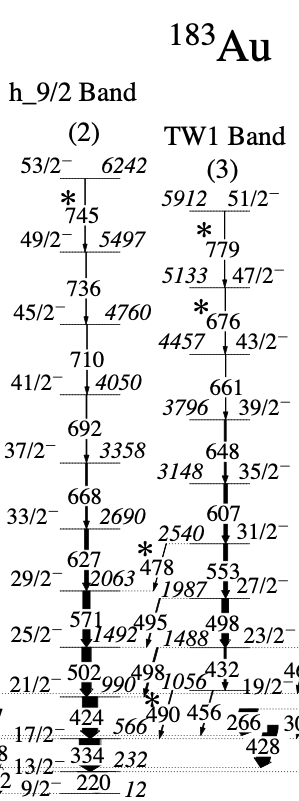
\includegraphics[scale=0.25]{figs/negative_Au183.png}%
    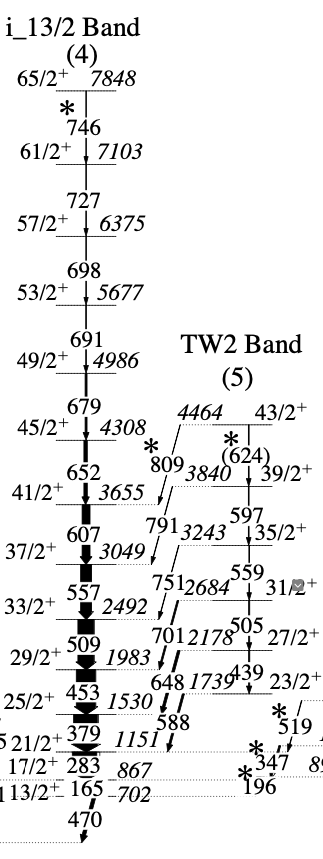
\includegraphics[scale=0.25]{figs/positive_Au183.png}
\end{figure}

\bibliography{references}

\end{document}